% SPDX-License-Identifier: CC-BY-SA-4.0
% SPDX-FileCopyrightText: Louis Royer <infos.louis.royer@gmail.com>
\documentclass[../main.tex]{subfiles}
\begin{document}
\initSubfile[2]
% utilisés uniquement pour la compilation isolée du chapitre (à mettre à jour en cas de changement)
\dummylabel{sec:MEC}{1.2.1}
\chapter{État de l'art des travaux intégrant de l'\textit{edge} dans la 5G}
\label{ch:state-of-the-art}
\begin{chapterHeader}
Ce chapitre dresse l’état de l’art des travaux permettant l’intégration de l’\textit{edge} dans la 5G.
En premier lieu, il définit nos exigences pour l’intégration de l’\textit{edge computing}, qui est l’un des pilier sur lequel reposera les prochaines générations de réseaux mobiles, et qui permettra l’émergence de nouvelles applications innovantes.
Ensuite, il présente les différents protocoles et architectures qui ont été publiés par les organismes de standardisation avant de faire la revue des travaux de recherche liés à l’\textit{edge computing}.
\end{chapterHeader}

\section{Exigences d’intégration}
\label{sec:exigences-integration}
Les caractéristiques de l’\textit{edge computing} rendent son intégration avec la 5G très désirable.
L’utilisation de l’\textit{edge computing} dans les réseaux~5G est nécessaire pour améliorer la \gl{QoE}{qualité d’expérience} des utilisateurs et permettre à des usages nouveaux d’émerger.
Selon nous, pour que cette intégration puisse être mise en œuvre dans des réseaux réels, elle doit garantir plusieurs propriétés.

\vspace{3cm}
\begin{figure}[h]
    \centering
    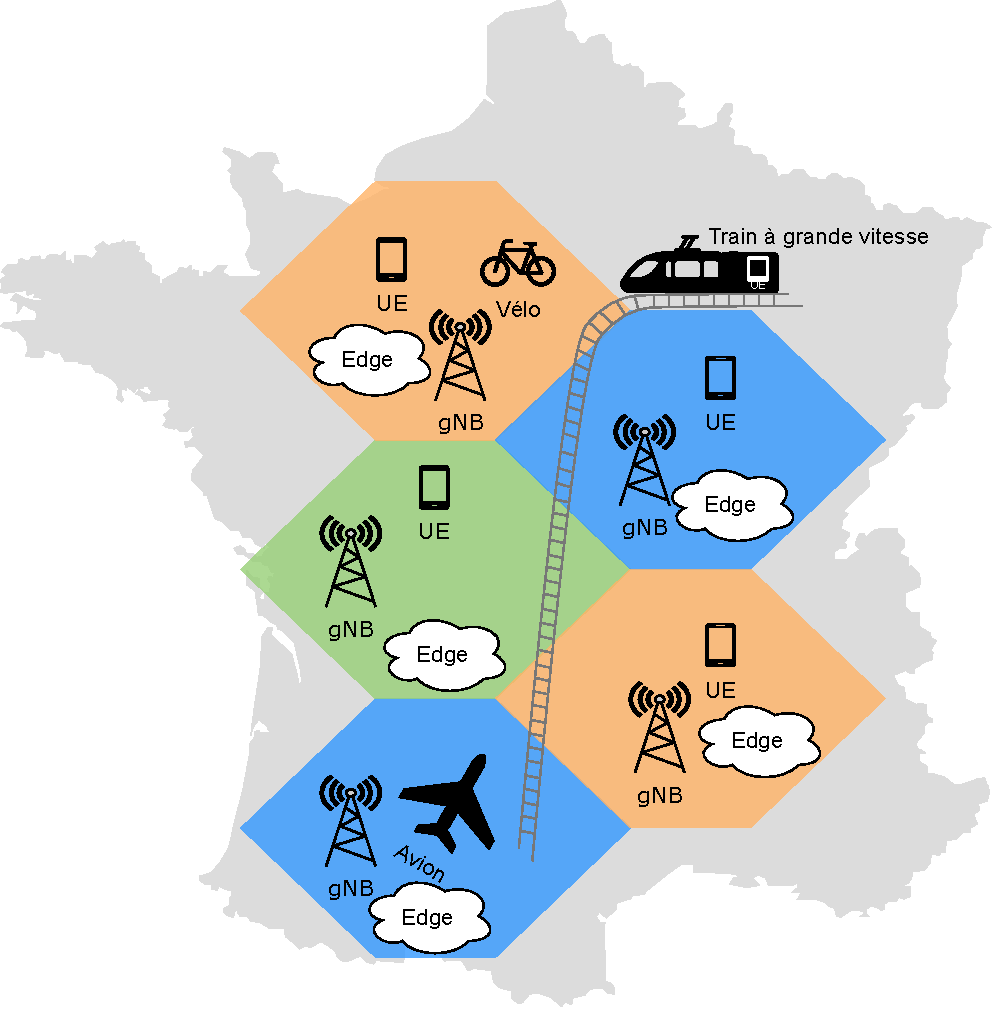
\includegraphics[width=0.75\linewidth]{figs/exigences_d_intégration.drawio.pdf}
    \caption[]{Nous considérons des réseaux de la taille d’un pays, dont les utilisateurs peuvent se déplacer très rapidement. Les opérateurs disposent généralement déjà d’infrastructures existantes qu’ils souhaitent faire évoluer à la fois pour proposer à leurs \gl{user}{abonnés} une meilleure \gl{QoE}{expérience utilisateur} et pour que le réseau soit géré de manière efficiente.}
    \label{fig:exigences-integration}
\end{figure}

\pagebreak
\subsection{Compatibilité avec les solutions existantes et passage à l’échelle}
Comme illustré sur la figure~\ref{fig:exigences-integration}, les réseaux mobiles font typiquement la taille d’un pays et ont un grand nombre d’utilisateurs qui accèdent à des services très variés.
La solution doit fonctionner malgré ces contraintes et doit anticiper les évolutions des usages. 

Les opérateurs existants disposent déjà d’infrastructures et si une solution d’intégration de l’\textit{edge computing} n’est pas compatible avec leur infrastructure, son adoption n’aura pas lieu.
Même si la virtualisation peut faciliter le déploiement d’une solution sur l’ensemble du réseau, il reste nécessaire que ce déploiement puisse s’effectuer sans interrompre le fonctionnement du réseau.

\subsection{Contrôle par l’opérateur et transparence pour l'utilisateur}
Pour que l’opérateur soit en mesure d’apporter des garanties sur la \gl{QoS}{qualité de service} au travers de \gl{SLA}{SLAs}, il est nécessaire qu’il dispose du contrôle sur la sélection des instances.
Cette sélection peut se faire suivant plusieurs critères (localisation, consommation, etc.) qui visent à une gestion intelligente des ressources de son réseau.
Puisque qu’il revient à l’opérateur de fournir l’accès au service demandé, ce processus doit pouvoir s’effectuer de manière invisible pour l’utilisateur.

Il existe une grande hétérogénéité entre les équipements utilisateur présents sur un réseau mobile.
Si la solution n’est pas indépendante de ce qui est ou ce qui n’est pas pris en charge par l’équipement, elle ne pourra pas avoir un succès à grande échelle. 

\subsection{Mobilité des utilisateurs et mise à jour dynamique}
Les utilisateurs des réseaux~5G sont toujours plus mobiles, et cette mobilité peut rendre la sélection initiale d’une instance non optimale.
Il est nécessaire que la solution soit en mesure de prendre en compte la mobilité en temps réel; cette mobilité peut avoir pour conséquence un changement d’instance utilisée.
Mais il est également possible que d’autres événements qu’une mobilité de l’utilisateur résultent en un changement d’instance 
(par exemple, lorsque des ressources temporairement indisponibles sont rétablies).

\subsection{Protection de la vie privée dès la conception}
Les systèmes modernes se doivent de respecter des principes qui favorisent la protection des données des utilisateurs.
L’opérateur connaît la localisation de l’utilisateur puisqu’il se connecte à son réseau par des équipements bien identifiés, cependant cette information n’était pas connue des fournisseurs de services dans le modèle du \textit{cloud computing}.
La solution d’intégration \textit{Edge}-5G donc doit limiter la capacité d’un service à connaître précisément la localisation des utilisateurs.

Pour cela il est nécessaire que la mise en relation entre l’utilisateur et l’instance d’un service soit faite entièrement par l’opérateur (qui peut alors combiner la localisation avec d’autres critères).
De même la solution doit offrir suffisamment de flexibilité pour qu’un utilisateur puisse être en mesure de s’opposer (par exemple, via son interface client) à tout moment à l’\gl{offloading}{\textit{offloading}} de ses données vers l’\gl{edge}{\textit{edge}}; il doit alors pouvoir utiliser une instance centrale des services même si cela implique qu’il ne bénéficie alors plus des avantages de cet \gl{offloading}{\textit{offloading}}.

\pagebreak
\section{Standardisation}
La standardisation est un processus qui favorise l’innovation et la recherche en créant une base commune pour le développement de nouvelles technologies, et leur adoption par l’industrie. C’est pourquoi plusieurs organismes de standardisation ont engagé des travaux visant à créer des systèmes interopérables pour intégrer l’\textit{edge computing} et la 5G.

\subsection{Intégration du \textit{Multi-access Edge Computing} (MEC) de l’ETSI}
L’\gl{ETSI}{ETSI} propose plusieurs scénarios de déploiement de son architecture \gl{MEC}{MEC} (présentée \hyperref[sec:MEC]{dans le chapitre précédent}), permettant son intégration avec des réseaux~5G.
L’infrastructure \acren{MEC} peut aussi bien être co-localisée avec la \gl{BS}{station de base} qu’être hébergée dans un \gl{datacenter}{centre de données} avec d’autres fonctions du cœur de réseau ou à des points d’agrégation intermédiaires (par exemple, dans un \gl{UPF}{UPF} local comme sur la figure~\ref{fig:ETSI-MEC-local-dn}).

\begin{figure}[h]
    \centering
    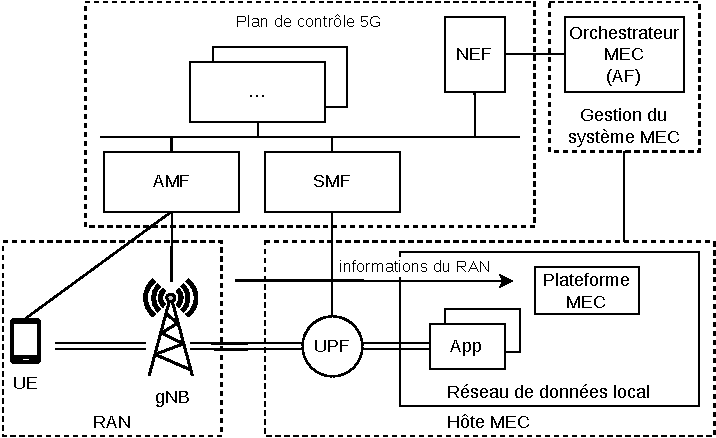
\includegraphics[width=0.9\linewidth]{figs/ETSI-MEC-local-dn.drawio.pdf}
    \caption[Intégration de l’architecture \textit{Multi-access Edge Computing} de l’ETSI avec la 5G]{Hôte MEC déployé dans un réseau de données local~\cite{ETSI.GR.MEC.WP.28}.}
    \label{fig:ETSI-MEC-local-dn}
\end{figure}

Dans tous ces scénarios, le système \acren{MEC} doit être en mesure d’\gl{TE}{orienter le trafic} vers les applications \acren{MEC}.
L’\acren{UPF} jouant un rôle central dans le routage, le groupe de travail considère qu’il est souhaitable que le système \acren{MEC} soit en mesure de configurer les \acrenpl{UPF} par l’intermédiaire d’une \gl{AF}{AF}~\cite{ETSI.GR.MEC.WP.28}.
Pour cela, l’\gl{ETSI}{ETSI} s’appuie sur le \acren{CAPIF}~\cite{3GPP.TS.23.222}, une \gl{API}{API} du \gl{3GPP}{3GPP}~\cite{ETSI.GR.MEC.031}.

Bien que standardisée, cette \gl{API}{API} n’est pas encore implémentée par la plupart des \gl{CN}{cœurs de réseau~5G} open-sources sur lesquels se basent la majorité des travaux de recherche~\cite{10.1007/978-3-030-49190-1_2}.
\pagebreak

\subsection{\textit{Edge} avec le standard 5G du 3GPP}
\subsubsection{\textit{Uplink Classifier} (ULCL)}
\label{sec:ULCL}
Dans le standard~5G, le mécanisme d’\acren{ULCL} permet de \gl{TE}{diriger le trafic (\textit{traffic steering})} suivant des règles~\gl{PFCP}{PFCP}~\cite{3GPP.TS.29.244} configurées par le \gl{SMF}{SMF} pour l’ensemble des~\acrenpl{UPF}~\cite{3GPP.TS.23.501}.

\begin{figure}[h]
    \centering
    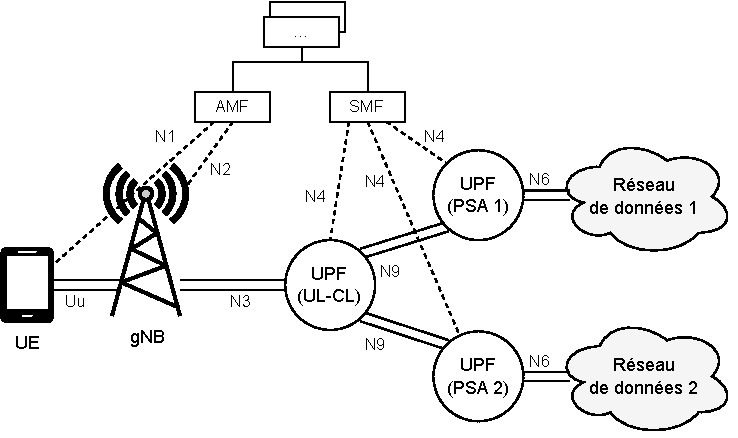
\includegraphics[width=0.9\linewidth]{figs/ULCL.drawio.pdf}
    \caption[Mécanisme d’\textit{Uplink Classifier}]{L’\acren{ULCL} peut \gl{TE}{diriger une partie du trafic} vers un réseau de données local~\cite{3GPP.TS.23.501}.} 
    \label{fig:ULCL}
\end{figure}

Cette solution, illustrée par la figure~\ref{fig:ULCL}, nécessite la configuration de chaque \acren{UPF} intermédiaire pour discriminer les \gl{PDU}{PDUs} suivant des règles prédéfinies.
Pour être en mesure de faire la différence entre plusieurs services, il est nécessaire pour les \acrenpl{ULCL} d’analyser en profondeur le contenu des \gl{PDU}{PDUs} puisque la couche~\gl{GTP}{GTP} ne contient que des informations sur le niveau de \gl{QoS}{qualité de service}, ainsi que des \gl{TEID}{identifiants de tunnels} qui correspondent à des \gl{PDU Session}{sessions PDU} sans distinction par service.
Pour pouvoir gérer un grand nombre de \gl{PDU Session}{sessions PDU}, il est nécessaire de grouper les règles redondantes grâce au mécanisme de \textit{PDI Optimization} car leur nombre a un impact sur le temps de traitement.
Cependant cette option n’est pas envisageable dès lors que l’on souhaite individualiser la sélection d’un \gl{edge}{\textit{edge}} pour un couple \gl{UE}{utilisateur}/\gl{service/instances}{service} selon des critères comme la pré-existence d’une session applicative.

Ce mécanisme fonctionne de manière complètement indépendante de l’\gl{UE}{équipement utilisateur} puisque sa mise en œuvre se déroule intégralement du côté du \gl{CN}{cœur de réseau}, cependant il complexifie la gestion de la continuité des sessions en cas de mobilité.
\pagebreak

\subsubsection{\textit{Multi-homing} IPv6}
Le \textit{multi-homing}~IPv6 est un second mécanisme proposé par le standard~5G permettant de fournir l’accès simultané à plusieurs \gl{DN}{réseaux de données}~\cite{3GPP.TS.23.501}.
Il consiste à associer plusieurs préfixes~IPv6 distincts à une \gl{PDU Session}{session PDU}: le trafic correspondant à chaque préfixe peut alors être dirigé vers un \gl{DN}{réseau de données} différent par un \gl{UPF}{UPF} intermédiaire en fondant sa décision sur le préfixe~IPv6 utilisé comme source dans la \gl{PDU}{PDU}.

Non seulement ce mécanisme nécessite que le cœur de réseau~5G, l’\gl{UE}{équipement utilisateur}, et l’ensemble des applications de ce dernier soit en mesure d’utiliser~IPv6, mais il est surtout indispensable que ces applications soient en mesure de sélectionner le meilleur préfixe selon la situation.

Ainsi ce mécanisme:
\begin{itemize}
    \item n’offre pas de contrôle à l’opérateur sur les chemins de données empruntés par les \gl{PDU}{PDUs}, ce qui rend cette solution inutilisable pour apporter des garanties de services;
    \item n’est pas utilisable de manière transparente par les applications, et n’est donc pas compatible avec celles qui ne sont pas conçues pour cet usage.
\end{itemize}

\subsection{Travaux de l’IETF}
\label{sec:ietf}
L’\acren{IETF} est l’organisme qui élabore la plupart des standards d’Internet.
Lorsqu’un sujet intéresse particulièrement la communauté, un groupe de travail est formé afin de rédiger et publier des brouillons (\textit{draft}) qui pourront être officialisés sous la forme de \acrenpl{RFC}~\cite{rfc2026}. 
Toutes les \acrenpl{RFC} ne sont pas des standards~\cite{rfc1796}: la plupart sont publiées à titre informatif, et il existe plusieurs niveaux de maturité pour les documents qui visent la standardisation.
Avant de devenir des standards, les \acrenpl{RFC} sont d’abord des « propositions de standards » (\textit{Proposed Standard}), puis des « brouillons de standards » (\textit{Draft Standards}).
Certaines \acrenpl{RFC} peuvent attendre plusieurs années avant de changer de niveau de maturité, et parfois même perdre leur statut et être classées comme « historiques » (y compris après la standardisation).

\subsubsection{\textit{Locator/ID Separation Protocol} (LISP)}
\label{sec:LISP}
L’espace d’adressage d’Internet est distribué par l’\acren{IANA} aux 5~\acrfrpl{RIR} qui le répartissent à leur tour entre plusieurs \gl{LIR}{registres locaux (\textit{Local Internet Registries}, LIRs)}.
Ces \acrenpl{LIR} assignent des blocs d’adresses~IP aux \acrfrpl{FAI} qui les utilisent pour leur infrastructure et en délèguent une partie à leurs clients.
Ces blocs d’adresses sont dits « \acren{PA} » car il est possible d’agréger les routes vers ces blocs d’adresses~IP, ce qui réduit le nombre d’entrées dans les tables de routage.
Avec cette méthode d’attribution, lorsqu’un \gl{user}{utilisateur final} change de \gl{FAI}{fournisseur d’accès}, il lui est nécessaire de changer toute la numérotation de ses équipements.
Il existe une deuxième catégorie de blocs d’adresses~IP, dits « \acren{PI} » qui sont assignés directement à l’utilisateur final par le \acren{RIR}.
La numérotation des équipements est alors indépendante du \gl{FAI}{fournisseur d’accès}, mais il n’est alors pas possible d’agréger les routes vers ces blocs d’adresses.

Cette deuxième méthode d’attribution a causé une croissance superlinéaire de la taille des tables de routages dans la \acren{DFZ} d’Internet, et pour y faire face il devient nécessaire de découpler la fonction d’identification des nœuds et la fonction de localisation au sein de la topologie.

\acren{LISP}~\cite{rfc9299,rfc9300} est donc proposé à la standardisation pour répondre à cette problématique; l’espace d’adressage y est séparé en deux: les \acrfrpl{EID} qui permettent aux équipements en bordure du réseau d’être identifiés indépendamment de leur localisation, et les \acrenpl{RLOC} qui sont agrégables et quasi-statiques~\cite{10.1109/MCOM.2015.7158286}. 

\begin{figure}[h]
    \centering
    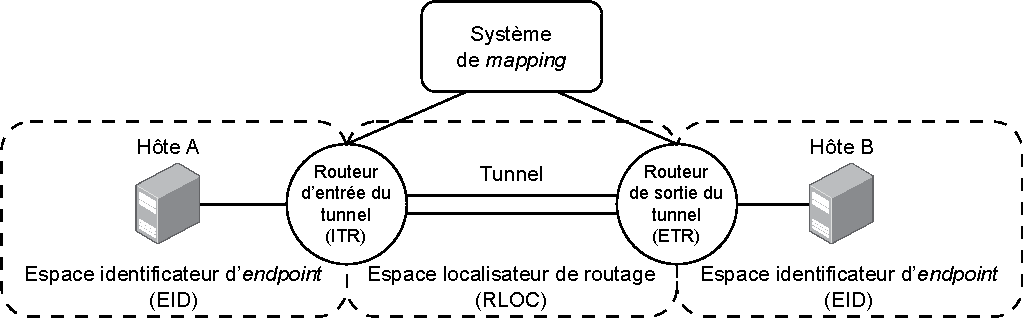
\includegraphics[width=0.70\linewidth]{figs/LISP.drawio.pdf}
    \caption[Architecture LISP]{Dans l’architecture de \acren{LISP}~\cite{rfc9299}, les adresses~IP des routeurs en bordure du réseau sont des \gl{RLOC}{localisateurs de routage}. Dans le \gl{CUPS}{plan de contrôle}, un système de \textit{mapping} associe les \gl{EID}{identifiants des \textit{endpoints}} à leur localisateur. Lorsque l’hôte~A communique avec l’hôte~B, les adresses utilisées par ces deux équipements sont uniquement des~\acrenpl{EID}.}
    \label{fig:LISP}
\end{figure}

Dans cette architecture, représentée sur la figure~\ref{fig:LISP}, pour relayer un paquet, les routeurs de bordures établissent des tunnels selon les informations qui lui sont fournies par un système de \textit{mapping}.
Ce système est une base de données distribuée dont l’interface est standardisée par l’IETF, et dont le fonctionnement peut s’appuyer sur le \gl{DNS}{DNS} ou sur d’autres technologies. 

Il est possible d’associer un \acren{EID} à plusieurs \acrenpl{RLOC}, ce qui permet une utilisation où un \acren{RLOC} correspond à une \gl{service/instances}{instance}, et un \acren{EID} à un \gl{service/instances}{service}.
Cependant, les critères de sélection de l’\gl{service/instances}{instance} se résument à des priorités et des poids qui sont appliqués par le routeur d’entrée de l’espace \acren{RLOC}.
Ce mécanisme est conçu pour permettre de faire de la répartition de charge et assurer la disponibilité du service en cas de panne d’une des \gl{service/instances}{instances}.
Il n’est pas possible de personnaliser cette sélection par d’autres critères que la localisation du routeur de bordure de la source.
Même si elle n’est par conséquent pas suffisante pour faire de l’\textit{edge computing}, cette architecture permet un déploiement progressif qui ne nécessite pas de changements dans le reste du réseau~\cite{10.1109/COMST.2017.2728478}.
L’architecture propose également un mécanisme qui permet de faire de l’\gl{TE}{ingénierie de trafic}: l’\acren{ELP} qui consiste à établir une succession de tunnels pour forcer le routage des paquets par certains localisateurs.

\acren{LISP} ne permet pas directement d’intégrer l’\textit{edge} dans la 5G car il lui manque en particulier tout l’aspect « gestion de la mobilité » (ce protocole ne traite pas la problématique de la continuité de service et de session) et que son mécanisme de mise en relation des hôtes ne permet pas une grande granularité.
Cependant, le concept d’une séparation par l’infrastructure réseau des fonctions de \gl{RLOC}{localisation} et \gl{EID}{identification} que \acren{LISP} propose semble indispensable à cette intégration.

\subsubsection{Routage par segment (\textit{Segment Routing})}
\label{sec:segment-routing}
Le \acrfr{SR} est une méthode de routage par la source qui consiste à marquer chaque paquet avec une liste d'instructions appelés segments. Chaque segment correspond à une \acrfr{VNF} implémentée au sein d’un nœud du réseau appelé \textit{endpoint}~\cite{rfc9256}.

Cette architecture permet de diriger les paquets suivant des politiques définies par le nœud d’entrée du domaine~\acren{SR} appelé \textit{headend} jusqu’à un nœud de sortie.
Ce \textit{headend} inscrit dans l’en-tête du paquet les \gl{SID}{identifiants des segments} intermédiaires à utiliser \gl{SID}{(\textit{Segment IDs}, SIDs)}.

Le \acrfr{SR} peut être déployé soit en utilisant un \gl{CUPS}{plan de données} \gl{MPLS}{MPLS (\textit{Multiprotocol Label Switching})}~\cite{rfc8660} soit en utilisant IPv6. Cette deuxième méthode est appelée \gl{SRv6}{SRv6 (\textit{Segment Routing over IPv6})}~\cite{rfc8986}. Par la suite, nous nous intéresserons uniquement à \acren{SRv6}.

Chaque \textit{endpoint} \acren{SRv6} peut implémenter plusieurs segments, et il existe des comportements standards qui permettent de faire de \gl{TE}{l’ingénierie de trafic (\textit{traffic-engineering})}. Par exemple, le comportement standard « \texttt{End} » consiste à transmettre le paquet au prochain \textit{endpoint} de la liste des segments après avoir décrémenté le compteur de segments restants. Sur la figure~\ref{fig:sr-behavior}, ce comportement est implémenté par les \textit{endpoints} \texttt{EP1} et \texttt{EP3}; on remarquera que la numérotation des fonctions n’est pas nécessairement identique pour tous les \textit{endpoints}. 

\begin{figure}[h]
    \centering
    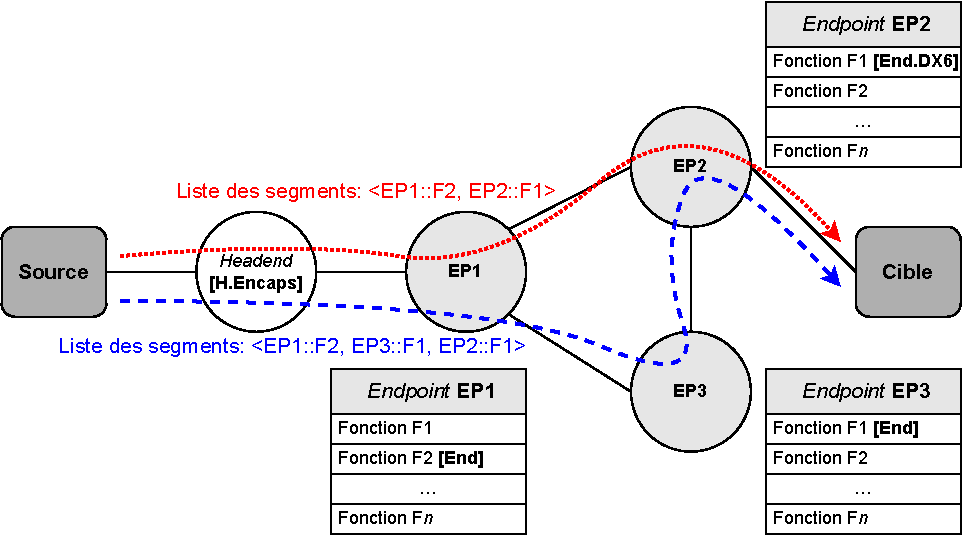
\includegraphics[width=0.7\linewidth]{figs/SR-behavior.drawio.pdf}
    \caption[Routage par segment avec SRv6]{Le \textit{headend} \texttt{H.Encaps} permet l’encapsulation de la charge utile dans un paquet IPv6. Deux politiques sont implémentées sur ce \textit{headend} (la politique rouge et la politique bleue). Les chemins correspondants à ces politiques se terminent tous les deux par la fonction \texttt{F1} de l’\textit{endpoint} \texttt{EP2}, qui implémente le comportement de dés-encapsulation (\texttt{End.DX6}).}
    \label{fig:sr-behavior}
\end{figure}

En \acren{SRv6}, les \acrenpl{SID} sont constitués de 128~bits, ce qui leur permet de correspondre chacun à une adresse IPv6. Cet identifiant est composé d’un préfixe, le \textit{locator}, qui permet d’identifier l’\textit{endpoint}, de l’identifiant d’une \gl{VNF}{fonction réseau} au sein de cet \textit{endpoint} et d’éventuels arguments que pourra utiliser cette fonction.

\pagebreak
La liste des \acrenpl{SID} est écrite dans une extension d’en-tête d’IPv6 dédiée au routage: le \acren{SRH}.
Il est également possible d’y associer un code d’\gl{HMAC}{authentification de message basé sur le hachage (\textit{Hash-based Message Authentication Code}, HMAC)}~\cite{rfc8754}. En effet, en SRv6 la connectivité entre certains \textit{endpoints} peut être apportée par l’intermédiaire de nœuds de transit ; ces derniers ne font pas partie du domaine~\acren{SR}, et il faut donc garantir qu’ils ne modifient pas la liste des segments.

\subsubsection{SRv6 pour le plan utilisateur des réseaux mobiles}
\label{sec:SRv6-MUP}
Le groupe de travail « \gl{DMM}{gestion distribuée de la mobilité} » de l’\gl{IETF}{IETF} \gl{DMM}{(\textit{Distributed Mobility Management}, DMM)}~\cite{IETF.DMM.HOMEPAGE} a travaillé sur une possible évolution du \gl{CUPS}{plan de données} des réseaux mobiles qui tire avantages des caractéristiques de \acren{SRv6}. La \gl{RFC}{RFC}~9433~\cite{rfc9433} (appelée \acren{SRv6}~\gl{MUP}{MUP}, pour \gl{MUP}{\textit{Mobile User Plane}}) donne les spécifications de nouveaux comportements d’\textit{endpoints} SRv6 à cet effet. Il ne s’agit néanmoins pas d’un standard, mais uniquement d’une \gl{RFC}{RFC} « pour information »: le groupe de travail estime qu’il est en dehors des attributions de l’IETF de standardiser les réseaux mobiles et que cette mission revient au \acren{3GPP}.

Le \acren{3GPP} avait déjà étudié en 2019 la possibilité de remplacer le \gl{CUPS}{plan de données} des réseaux mobiles par \acren{SRv6}, mais avait décidé de ne pas le standardiser~\cite{3GPP.TR.29.892}. Il reste cependant envisageable que les nouveaux problèmes de \gl{scalability}{passage à l’échelle} soulevés par l’usage du \acren{MEC} ou que des cas d’usage comme le \acrfr{SFC}~\cite{rfc7665}, ou le \textit{Computing Power Network}~\cite{10.1109/CCET55412.2022.9906338}, que le \gl{3GPP}{3GPP} n’avait pas considéré jusqu’alors, le motive à ré-examiner cette possibilité.

Le périmètre de cette \gl{RFC}{RFC} se limite au \gl{CUPS}{plan de données}. Pourtant, il est nécessaire de modifier le protocole de contrôle pour permettre la définition des différentes politiques~\acren{SR}~\cite{10.1109/ICTC55196.2022.9953021}.

La \gl{RFC}{RFC}~9433 propose deux modes de fonctionnement: un mode dit « traditionnel » qui permet de remplacer \gl{GTP}{GTP-U} par \acren{SRv6} sans effectuer d’autres changements, et un mode « amélioré » qui permet d’utiliser pleinement les fonctionnalités de \acren{SRv6} notamment pour l’ingénierie de trafic. Trois mécanismes d’interopérabilité sont également définis pour fonctionner respectivement avec des \acrenpl{gNB} utilisant \gl{GTP}{GTP-U} sur IPv4, des \acrenpl{gNB} utilisant \gl{GTP}{GTP-U} sur IPv6, et d’autres \acrenpl{UPF} n’utilisant pas \acren{SRv6}.

\begin{figure}[h]
    \centering
    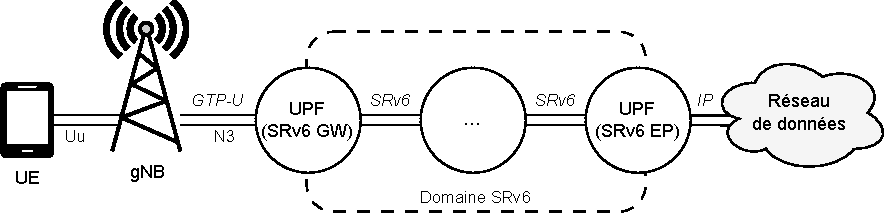
\includegraphics[width=0.80\linewidth]{figs/SRv6-MUP.drawio.pdf}
    \caption[SRv6 pour le plan utilisateur des réseaux mobiles (SRv6 MUP)]{SRv6 pour le \gl{CUPS}{plan utilisateur} des réseaux mobiles, avec son mécanisme d’interopérabilité « \acren{gNB} non-modifiée utilisant \gl{GTP}{GTP-U} sur IPv4 »~\cite{rfc9433}.}
    \label{fig:SRv6-MUP}
\end{figure}

Nous nous intéresserons particulièrement à ce premier mécanisme d’interopérabilité dans le mode « amélioré » (voir figure~\ref{fig:SRv6-MUP}) qui est particulièrement pertinent pour des déploiements à partir de réseaux existants puisqu’il permet d’effectuer du \gl{TE}{\textit{traffic steering}} tout en conservant le \gl{RAN}{RAN} inchangé.
\pagebreak

Afin de permettre la traduction entre \acren{SRv6} et \gl{GTP}{GTP-U}, un conteneur \texttt{Args.Mob.Session} de 40~bits est créé pour transporter les informations relatives à la \gl{PDU Session}{session PDU} telles que le \gl{TEID}{numéro de tunnel (TEID)} et les paramètres de \gl{QoS}{qualité de service}. Pour le scénario qui nous intéresse, la \gl{RFC}{RFC} a défini deux nouveaux comportements qui sont présentés dans le tableau~\ref{table:func-SRv6-MUP}.

Puisque ces nouveaux comportements sont conçus pour permettre l’interconnexion avec des équipements \acren{GTP}, les \acrenpl{SID} manipulés comprennent également une adresse IPv4 encodée en tant qu’argument: elle correspond à l’adresse de l’équipement auquel transmettre le paquet \acren{GTP} créé en sortie du domaine \acren{SRv6} et est nécessaire pour obtenir un numéro de tunnel globalement unique, c’est-à-dire un numéro de tunnel entièrement qualifié (\textit{Fully-qualified \gl{TEID}{Tunnel Endpoint Identifier}}, FTEID).

\begin{table}[h]
\centering
\scalebox{0.9}{
\begin{tabular}{cc}
\toprule
\thead{Comportement} & \thead{Description}  \\
\midrule
\texttt{End.M.GTP4.E}  & Traduction de \acren{SRv6} vers « \gl{GTP}{GTP-U} sur IPv4 » \\
\texttt{H.M.GTP4.D}    & Traduction de « \gl{GTP}{GTP-U} sur IPv4 » vers \acren{SRv6} \\
\bottomrule
\end{tabular}
}
\caption[Comportements SRv6 pour le plan de données utilisateur des réseaux mobiles]{Dans le mode « amélioré », et avec le mécanisme d'interopérabilité « \acren{gNB} non-modifiée utilisant \gl{GTP}{GTP-U} sur IPv4 », seuls deux nouveaux comportements \acren{SRv6} sont nécessaires. Il existe des comportements similaires pour fonctionner avec « \gl{GTP}{GTP-U} sur IPv6 ».}
\label{table:func-SRv6-MUP}
\end{table}

Les analyses de performances du \gl{CUPS}{plan de données} mobile avec \acren{SRv6} montrent qu’il n’y a pas de surcoût significatif en terme de débit par rapport à \gl{GTP}{GTP-U}~\cite{10.1109/ACCESS.2024.3418960}, et que les \textit{frameworks} modernes tel que \gl{VPP}{VPP (\textit{Vector Packet Processor})} permettent de faire les conversions entre \acren{SRv6} et \gl{GTP}{GTP-U} (et vice-versa) en limitant le surcoût en terme de latence à un intervalle entre 3 et \SI{30}{\micro\second}~\cite{10.1109/COMPSAC51774.2021.00212}.

\section{Problématiques liées à l’\textit{edge computing}}
Dans cette section, nous aborderons diverses problématiques liées à l’\textit{edge computing}. Nous commencerons par proposer une vue d’ensemble des travaux sur l’intégration du \gl{MEC}{MEC} avec le \gl{RAN}{réseau d’accès radio} de la 5G, puis nous nous concentrerons sur les problématiques liées au cycle de vie des instances d’un service MEC: le placement des instances et la gestion de ce cycle de vie, leur migration, mais également la mise en relation d’un utilisateur avec un instance avant un accès effectif à celles-ci.

\subsection{Intégration du MEC avec le RAN}
\subsubsection{Vue d’ensemble}
De nombreux travaux visent à mieux intégrer le \gl{MEC}{MEC} avec le \gl{RAN}{RAN}~5G afin de tirer profit des ressources qu’il met à disposition.
Dans cette section, nous proposons une vision globale de ces différentes approches. Tout d’abord, nous aborderons brièvement les perspectives offertes par l’intégration avec l’architecture \gl{O-RAN}{O-RAN} que nous avions décrite dans le chapitre précédent. Nous montrerons ensuite les perspectives offertes par le \acren{D2D} et par l’accès multiple non-orthogonal.
Enfin, nous envisagerons l’intégration avec le \gl{RAN}{RAN} \gl{NTN}{non-terrestre}, qui constituera très probablement l’un des sujets de recherche clés de la prochaine génération de réseaux mobiles.

\pagebreak
\subsubsection{Intégration avec O-RAN}
Certains travaux proposent d’intégrer le \gl{MEC}{MEC} avec l’architecture \gl{O-RAN}{O-RAN}~\cite{10.1109/MNET.2020.9277891,10.1109/WCNC57260.2024.10571112}.
Dans ces approches, les ressources \gl{MEC} sont disposées au plus près des \gl{BS}{stations de base}, comme illustré par la figure~\ref{fig:integration-oran}, et ce sont ces dernières qui vont décider d’effectuer ou non un \gl{offloading}{\textit{offloading}} des tâches.

\begin{figure}[h]
    \centering
    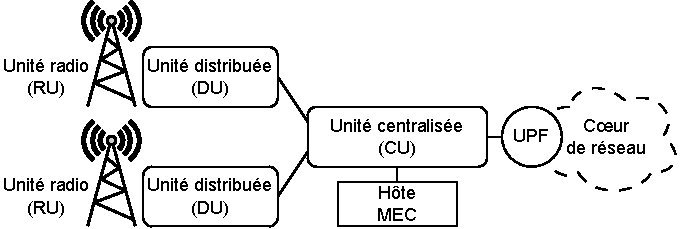
\includegraphics[width=0.85\linewidth]{figs/integration-oran.drawio.pdf}
    \caption[Architecture O-RAN]{Dans ce modèle d’intégration, ce ne sont pas les \gl{UPF}{UPFs} qui dirigent le trafic vers les hôtes~\gl{MEC}{MEC}, mais l’\gl{CU/DU}{unité centralisée}~\cite{10.1109/WCNC57260.2024.10571112}.}
    \label{fig:integration-oran}
\end{figure}

Cette intégration permet également aux services \gl{MEC}{MEC} de bénéficier de nouvelles \gl{API}{APIs} spécifiques au \gl{RAN}{RAN}, telles que des fonctions de localisations.

\subsubsection{Intégration avec le \textit{device-to-device} (D2D)}
Le \gl{D2D}{\textit{device-to-device}} est un mode de communication où les \gl{UE}{équipements utilisateur} sont en capacité de communiquer entre eux sans l’intermédiaire de la \gl{BS}{station de base}~\cite{10.1109/ACCESS.2021.3063104}. Ces communications peuvent être orchestrée par le réseau, qui sert uniquement au contrôle (signalisation, gestion des ressources radio, etc.) ou être gérée de manière autonome. 
Ce premier scénario est très coûteux en terme de messages de contrôle lorsque de nombreux appareils souhaitent communiquer, et réduit l’efficacité spectrale. Le deuxième scénario évite le problème du coût des messages de contrôle, mais cause des instabilités dans les communications.
Il existe donc un troisième scénario, qui fait un compromis entre les deux scénarios précédents: l’infrastructure réseau s’occupe de la signalisation et de l’établissement des nouvelles connexions, mais délègue la gestion des ressources radio aux équipements.

Pour certains usages, il est possible d’étendre le modèle du \gl{MEC}{MEC} pour faire de l’\gl{offloading}{\textit{offloading}} de tâches vers des \gl{UE}{équipements}, qui peuvent alors être considérées comme des ressources \gl{MEC}{MEC}. Par exemple, certains travaux proposent de fournir des points d’accès aériens par l’intermédiaire de drones~\cite{10.1109/TVT.2025.3540915}.
Leur capacité à se déplacer rend pertinent leur statut d’« \gl{UE}{équipement utilisateur} », puisqu’ils ne disposent pas d’un lien filaire pour se connecter à un \gl{UPF}{UPF}, mais peuvent en revanche bénéficier du lien radio~5G pour se raccorder au reste du réseau.

\pagebreak
\subsubsection{Intégration avec l’accès multiple non-orthogonal (NOMA)}
L’accès multiple non-orthogonal (\textit{Non-Orthogonal Multiple Access}, NOMA) permet à plusieurs utilisateurs de partager les mêmes ressources radio en les séparant via leur puissance d’émission plutôt que par des créneaux temporels ou une division fréquentielle~\cite{10.1109/ACCESS.2020.3001277,10.1109/ACCESS.2023.3326846}. Cette technique utilise des codes de superposition (\textit{Superposition Coding}, SC) en émission et de l’annulation successive d’interférence (\textit{Successive Interference Cancellation}, SIC) en réception pour discriminer les signaux.

Ce partage de ressources radio permet à la fois d’optimiser l’usage du spectre, mais également de gérer plus efficacement le déchargement vers des hôtes \gl{MEC}{MEC}, comme l’illustre la figure~\ref{fig:NOMA-uplink-downlink}.

\vspace{1.5cm}
\begin{figure}[h]
    \centering
    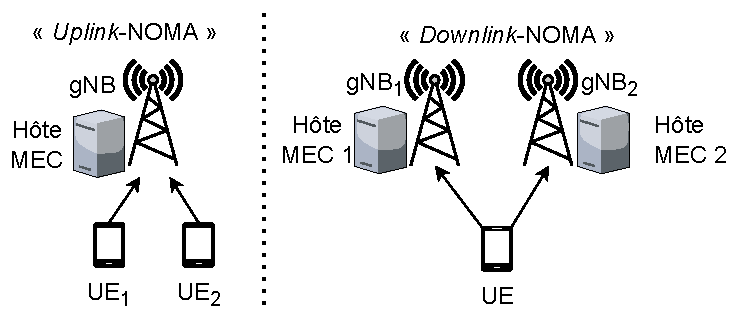
\includegraphics[width=0.80\linewidth]{figs/NOMA-Uplink-Downlink.drawio.pdf}
    \caption[Accès multiple non-orthogonal (NOMA)]{L’\textit{Uplink}-NOMA permet à plusieurs utilisateurs d’émettre à destination d’un seul hôte MEC en utilisant les mêmes ressources radio. Le \textit{Downlink}-NOMA correspond à la situation inverse: un utilisateur émet vers plusieurs hôtes MEC qui se partagent les mêmes ressources radio. Ici, les termes « \textit{Uplink} » et « \textit{Downlink} » ne font contre-intuitivement pas référence au sens de la communication (lien montant et lien descendant), puisque l’\gl{offloading}{\textit{offloading}} se fait toujours dans le sens montant (dans sa signification usuelle).}
    \label{fig:NOMA-uplink-downlink}
\end{figure}

\subsubsection{Intégration avec le RAN non-terrestre}
Les constellations de satellites en \gl{LEO}{orbite basse (\textit{Low Earth Orbit}, LEO)} offrent une faible latence et une large couverture du globe.
Avec l’intégration des \gl{NTN}{réseaux non-terrestres} aux réseaux mobiles, embarquer des serveurs \gl{MEC}{MEC} comme charge utile de ces constellations \gl{LEO}{LEO} permettrait de bénéficier de capacités MEC de manière ubiquitaire~\cite{10.1109/COMST.2025.3534617}. De plus, dans les scénarios où l’accès par satellite est l’unique méthode d’accès au réseau mobile, l’usage d’un \gl{MEC}{MEC} intégré au \gl{RAN}{RAN} \gl{NTN}{non-terrestre} évite à une partie des communications d’avoir à traverser l’ensemble de la constellation pour joindre un \gl{datacenter}{centre de données} terrestre, réduisant ainsi les coûts en termes de débit et de latence~\cite{10.1109/AERO63441.2025.11068449}.

\pagebreak
\subsection{Problème du placement des instances et gestion de leur cycle de vie}
\label{sec:placement-instances}
\subsubsection{Problématique}
La gestion des ressources vise à respecter les \acrfrpl{SLA} tout en minimisant les coûts, qui peuvent englober aussi bien le prix de déploiement (construction, achats de matériel) que celui de fonctionnement (énergie)~\cite{10.1109/JIOT.2021.3082898}.
Cette gestion commence par le choix de la localisation des infrastructures d’\textit{edge computing}.
Des \gl{service/instances}{instances} y sont continuellement déployées, migrées, ou détruites tout le long du cycle de vie des \gl{service/instances}{services} en fonction des usages des utilisateurs, comme illustré sur la figure~\ref{fig:problème-du-placement-des-instances}.

\vspace{1.5cm}
\begin{figure}[h]
    \centering
    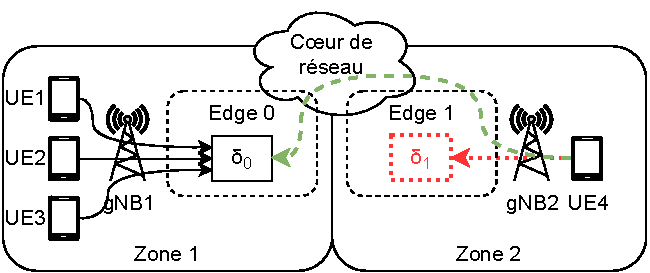
\includegraphics[width=0.9\linewidth]{figs/instance-placement-problem.drawio.pdf}
    \caption[Placement des instances]{Selon les contraintes de l’application, lorsque l’UE4 souhaite accéder au service $\Delta$, plutôt que de déployer une instance locale $\delta_1$, il peut être plus judicieux d’agréger tous les utilisateurs sur une instance $\delta_0$ d’un \gl{edge}{\textit{edge}} voisin afin de réduire la consommation globale de ressources.}
    \label{fig:problème-du-placement-des-instances}
\end{figure}
\vspace{1.5cm}

Ces \gl{service/instances}{instances} vont ensuite être réparties entre les utilisateurs d’un \gl{service/instances}{service} afin d’atteindre les objectifs fixés, qui peuvent être différents selon les \gl{service/instances}{services} et les utilisateurs:
par exemple, des contraintes temporelles (latence), énergétiques, ou de taux d’utilisation des ressources (processeurs, mémoire, bande passante, etc.)~\cite{10.1109/JIOT.2021.3082898,10.1145/3592598}.

Comme le placement des instances est un problème d’optimisation combinatoire \gl{NP-Hard}{NP-difficile}, de nombreuses approches ont été proposées~\cite{10.1145/3729214}.
Ces propositions reposent généralement sur des méthodes d’apprentissage, sur des méta-heuristiques, ou sur des modèles statistiques~\cite{10.1109/TNSM.2024.3375970}.

\pagebreak
\subsubsection{Modes de placement}
Il existe deux familles de stratégies pour la coordination du placement: les stratégies centralisées, et les stratégies distribuées~\cite{10.1145/3391196}. La plupart des travaux utilisent des stratégies centralisées car les stratégies distribuées ne permettent que d’obtenir un optimal local, sans garantie sur l’optimalité globale.
Cependant, les stratégies distribuées permettent un meilleur \gl{scalability}{passage à l’échelle} en réduisant la complexité algorithmique.
Elles facilitent également l’intégration dans le \gl{CUPS}{plan de contrôle} de la~5G en autorisant un \gl{scalability}{passage à l’échelle} horizontal de la \gl{NF}{fonction réseau} chargée de cette coordination.

Le placement peut être statique ou dynamique: dans le premier cas, il est possible de faire un calcul hors-ligne du placement ce qui permet d’obtenir de meilleures optimisations en assouplissant les contraintes temporelles pour l’obtention d’une solution; dans le cas cas dynamique, on peut en revanche prendre en compte les évolutions dans le système telles que la mobilité des utilisateurs.

Dans le cas d’un placement dynamique, il existe deux modes de placement: un mode proactif et un mode réactif.
Dans le mode réactif, les changements dans le choix du placement seront déclenchés par le dépassement d’un seuil, par exemple lorsqu’une instance est surchargée.
Dans le mode proactif, on cherchera à anticiper le comportement du système, par exemple en prédisant qu’un \gl{handover}{\textit{handover}} va être effectué.

\subsubsection{Formulation du problème et méthodes de résolution}
Le problème du placement des instances est formulé comme un problème d’optimisation.
Généralement, il s’agit d’une optimisation multi-objectifs: par exemple, on va chercher à satisfaire à la fois des contraintes d’énergie et de latence.
Puisqu’il n’est pas possible de satisfaire simultanément toutes les contraintes, plusieurs approches existent.
Dans cette situation, une première approche consiste à chercher un optimum de Pareto, c’est-à-dire chercher une solution où il n’est plus possible d’améliorer le résultat sur un critère sans dégrader son optimalité selon les autres critères.
Une seconde approche consiste à faire une scalarisation linéaire pour ramener le problème à un problème simple-objectif, en donnant un poids à chaque contrainte.

Dans la littérature, les formulations sont variées: \gl{ILP}{optimisation linéaire en nombres entiers (\textit{Integer Linear Programming}, ILP)}, \gl{NLP}{optimisation non linéaire (\textit{Non-Linear Programming}, NLP)}, modèle s’appuyant sur la théorie des jeux, sur la théorie des graphes, etc.
Chaque modèle offre une gamme différente de méthodes et d’outils permettant la résolution~\cite{10.1109/COMST.2021.3101460}.

Par exemple, dans le cadre de la résolution de problèmes d’optimisation linéaire en nombres entiers, il est possible d’utiliser un \gl{B-and-B}{algorithme de séparation et évaluation (\textit{Branch and Bound}, B\&B)} pour obtenir une solution exacte.
Cependant toutes les tentatives de résolutions exactes sont coûteuses en pratique, et cette approche ne fait pas exception: la résolution d’\gl{ILP}{ILP} est connue pour être \gl{NP-Hard}{NP-difficile}.

Des méthodes d’approximation permettent d’accélérer la résolution.
L’approche de référence consiste à relâcher la contrainte d’intégralité pour obtenir un \gl{LP}{problème d’optimisation linéaire (\textit{Linear Programming}, LP)} que l’on peut ensuite résoudre de manière exacte avec l’algorithme du simplex afin de guider la construction d’une solution pour le problème original.

\pagebreak
La résolution de problèmes d’optimisation non-linéaire pose le même type de problématiques.
On préférera donc généralement se contenter d’optimums locaux avec des algorithmes comme \gl{SPQ}{SQP (\textit{Sequential Quadratic Programming})}, même si le recourt à des schémas globaux (\gl{B-and-B}{B\&B} spatial avec relaxations convexes), eux aussi coûteux, reste envisageable.

Plus récemment, de nouvelles approches émergent: elles sont basées sur l’\gl{DRL}{apprentissage par renforcement profond (\textit{Deep Reinforcement Learning}, DRL)}.
Celles-ci peuvent intervenir à la fois dans la construction de solutions aux différents modèles (\textit{model-based approach}) ou se passer complètement de modélisation (\textit{model-free approach}).

\subsection{Migration d’instances}
\subsubsection{Problématique}
Au cours du cycle de vie d’une session applicative, il est possible qu’un évènement force une migration de cette session vers une nouvelle instance, par exemple en cas de mobilité de l’utilisateur.
Cette instance peut soit être nouvellement déployée dans un \gl{edge}{\textit{edge}}, comme décrit dans la section précédente, soit être déjà existante (voir figure~\ref{fig:container-vs-session-migration}).

\begin{figure}[h]
    \centering
    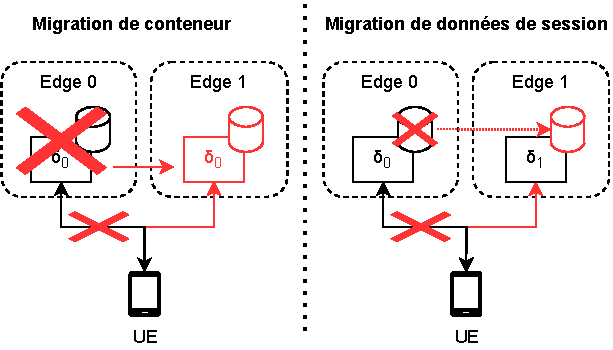
\includegraphics[width=0.9\linewidth]{figs/container-vs-session-migration.drawio.pdf}
    \caption[Migration d’instance]{Lorsque le service n’est pas déployé dans l’\gl{edge}{\textit{edge}} cible, la migration de conteneur (ou de machine virtuelle) permet de migrer l’ensemble des sessions en cours avec ce service; avec cette méthode la migration peut être menée entièrement par l’orchestrateur, indépendamment de l’application. Lorsqu’il existe déjà une instance dans l’\gl{edge}{\textit{edge}} cible, il est possible de migrer individuellement les sessions; mais le service doit alors être conçu de telle sorte à rendre cette migration possible.}
    \label{fig:container-vs-session-migration}
\end{figure}

\pagebreak
Afin de permettre un changement transparent pour l’utilisateur et d’éviter une interruption de service, si celui-ci comporte des états il est nécessaire de les transférer vers l’instance cible.
Les états à migrer peuvent être des données applicatives, ou des données de transport (numéro de séquence de segments, clé de chiffrement \gl{TLS}{TLS}, etc.).

Il existe plusieurs stratégies pour effectuer cette migration: les deux principales sont la copie \textit{a priori}, et la copie \textit{a posteriori}~\cite{10.1109/ACCESS.2018.2828102}. Il est possible d’utiliser un stratégie hybride, mais elle hérite alors des défauts des deux méthodes principales~\cite{10.1145/3704436}.

\subsubsection{Copie \textit{a priori}}
\label{sec:migration-copie-a-priori}
La copie \textit{a priori} consiste à garder en fonctionnement l’instance cible jusqu’au changement effectif d’instance. Lorsque le processus de migration commence, les données sont synchronisées vers l’instance cible qui reste en fonctionnement jusqu’à ce qu’un niveau de synchronisation suffisant soit atteint. Lorsque la migration peut être achevée dans un délai acceptable, l’infrastructure peut déclencher le changement effectif d’instance, et les nouvelles requêtes seront placées dans la file d’attente de l’instance cible jusqu’à ce qu’elle soit en mesure de les traiter, ce qui peut éventuellement mener à une dégradation temporaire de la \gl{QoS}{qualité de service}.

Cette méthode est coûteuse en temps de migration puisque des données qui avaient déjà été transférées peuvent évoluer dans l’instance source, et qu’il faut alors répliquer cette évolution dans l’instance cible. Prioriser la transmission des ressources les moins susceptibles d’évoluer permet de réduire ce risque. Cette méthode a l’avantage de permettre un mode de fonctionnement sans interruption de service sous réserve que la valeur de référence choisie pour le niveau de synchronisation soit suffisamment élevée, mais elle n’est utilisable que lorsque la migration a été anticipée. 

\subsubsection{Copie \textit{a posteriori}}
À l’opposé de cette méthode, la copie \textit{a posteriori} gèle immédiatement les données de l’instance source, effectue la copie, puis déclenche le changement effectif d’instance.

Cette méthode nécessite moins de temps et moins de bande passante puisqu’il ne sera jamais nécessaire de transmettre plusieurs fois la même donnée, mais elle implique obligatoirement une interruption de service.
En conséquence, il faut réserver cette méthode aux situations où une interruption de service a déjà eu lieu (perte temporaire du lien radio) ou est inévitable car la migration n’a pas pu être anticipée assez tôt. Par exemple en cas de coupure de la source d’alimentation électrique principale dans un \gl{edge}{\textit{edge}}, la migration des données, puis l’arrêt des équipements seront déclenchés en urgence avant l’extinction de l’alimentation de secours.

\pagebreak
\subsection{Mise en relation et accès aux instances} 
\subsubsection{Vue d’ensemble}
Pour permettre aux \gl{UE}{équipements utilisateurs} d’utiliser un \gl{service/instances}{service}, il convient de choisir une \gl{service/instances}{instance} à utiliser et de faire le nécessaire afin que les \gl{PDU}{PDUs} puissent être échangées entre l’\gl{UE}{UE} et l’\gl{service/instances}{instance} sélectionnée.

\begin{figure}[h]
    \centering
    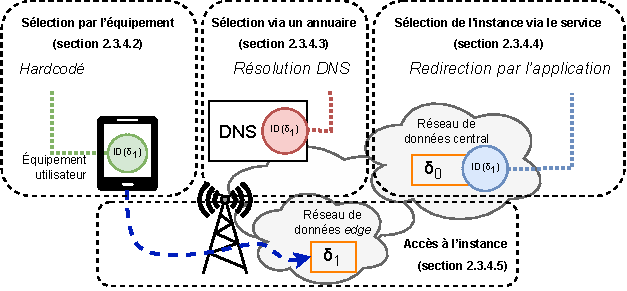
\includegraphics[width=0.8\linewidth]{figs/mise-en-relation.drawio.pdf}
    \caption[Méthodes de mise en relation et d’accès aux instances]{La mise en relation peut être implémentée directement au niveau de l’équipement utilisateur, lors de la résolution du nom de domaine, ou dans une instance centrale de l’application.}
    \label{fig:mise-en-relation}
\end{figure}

Les méthodes existantes, illustrées par la figure~\ref{fig:mise-en-relation}, sont issues du paradigme du \textit{cloud computing} et reposent donc toutes directement ou indirectement sur la pré-existence d’un chemin vers l’instance sélectionnée.
Cette instance peut se situer dans un \gl{edge}{\textit{edge}} local ou être accessible via le réseau de données principal.

Ces méthodes rendent coûteuses l’utilisation d’une instance située dans un \gl{edge}{\textit{edge}} distant (suite à une mobilité par exemple), car elles forcent alors un routage passant par le \gl{PSA}{PSA}.
Aucune de ces méthodes n’est complètement transparente pour l’\gl{UE}{équipement utilisateur}, puisqu’à l’issue du processus de sélection, il indique l’adresse de l’instance choisie dans l’en-tête des \gl{PDU}{PDUs} qu’il envoie.

\subsubsection{Sélection autonome de l’instance par l’équipement utilisateur}
Lorsque le \gl{service/instances}{service} ne dispose que d’un nombre limité d’\gl{service/instances}{instances} qui n’est pas susceptible d’évoluer, il est possible pour l’application de l’équipement utilisateur de déterminer de manière autonome quelle instance sélectionner.
Ce choix est alors vraisemblablement statique, et ne peut se faire que sur un nombre limité de critères grâce à une connaissance préalable de la topologie du réseau et une liste pré-établie des adresses des \gl{service/instances}{instances} existantes.

Avec cette méthode, il est impossible de garantir que l’instance sélectionnée est optimale, et les informations connues de l’application risquent de ne plus être exactes sur le long terme.

\pagebreak
\subsubsection{Sélection de l’instance via un annuaire}
Pour obtenir l’adresse d’un hôte dont on ne connaît qu’un nom symbolique, il est possible de consulter un annuaire, par exemple~\gl{DNS}{DNS}.
Lorsque le choix de l’instance n’a aucune importance, ce système permet d’obtenir l’adresse d’une ou plusieurs \gl{service/instances}{instances} d’un \gl{service/instances}{service}, au prix d’une communication avec le réseau.
Il est possible pour l’infrastructure réseau de diriger les requêtes~\gl{DNS}{DNS} vers un résolveur local afin de réduire l’impact de cette communication.

Pour sélectionner la meilleure instance pour un équipement à un instant donné, il existe deux approches qui nécessitent toutes les deux une collaboration entre l’opérateur réseau et le fournisseur du \gl{service/instances}{service}.

La première approche consiste à faire mentir le résolveur~\gl{DNS} utilisé par l’\gl{UE}{UE} afin que sa réponse soit adaptée à la situation de l’équipement. Si le fournisseur du \gl{service/instances}{service} utilise \gl{DNSSEC}{DNSSEC}~\cite{rfc9364} qui vise justement à ce que les résolveurs~\gl{DNS} ne puissent pas mentir à l’utilisateur, le fournisseur du \gl{service/instances}{service} doit alors déléguer une zone~\gl{DNS}{DNS} à l’opérateur.
Cette pratique semble difficilement compatible avec la possibilité de fournir ce \gl{service/instances}{service} via plusieurs opérateurs simultanément. Les alternatives sont de ne pas utiliser \gl{DNSSEC}{DNSSEC} ou de fournir une copie de la clé privée de signature de zone à l’opérateur: aucune de ces solutions n’est raisonnablement envisageable car elles brisent le modèle de sécurité.

La deuxième approche consiste à utiliser \acren{EDNS Client Subnet}~\cite{rfc7871} pour que le serveur \gl{DNS}{DNS} faisant autorité obtienne l’adresse de l’\gl{UE}{équipement utilisateur} et puisse adapter sa réponse après avoir demandé à l’opérateur des informations sur cet \gl{UE}{équipement} (par exemple, sa localisation). Cette approche n’est pas compatible avec l’ensemble des \gl{UE}{UEs} car \acren{EDNS Client Subnet} est une extension de \gl{DNS}{DNS} qui n’est pas obligatoirement implémentée sur tous les équipements, et qui peut être désactivée par l’utilisateur. De plus cette approche présente des risques pour la vie privée de l’utilisateur puisqu’elle permet au fournisseur de service, par conception, d’obtenir des informations sur l’utilisateur qu’il ne devrait habituellement pas connaître.

Quelle que que soit l’approche retenue, la sélection de l’instance via un annuaire semble difficilement compatible avec un usage mobile de l’\textit{edge computing}:
afin d’éviter de surcharger le réseau avec une résolution~\gl{DNS}{DNS} pour chaque émission de paquet, les informations obtenues via ce système sont assorties d’une durée de vie.

Pendant toute la durée de vie de l’information, celle-ci peut être mise en cache par l’équipement utilisateur qui ne pourra alors pas mettre à jour l’instance sélectionnée avant que ce cache soit invalidé. Définir une durée de vie trop courte ne permet pas le passage à l’échelle avec le nombre d’utilisateurs et d’applications, et n’est de toute manière pas une condition suffisante pour garantir la sélection et l’utilisation immédiate d’une instance éventuellement différente en cas de mobilité.

\pagebreak
\subsubsection{Sélection de l’instance via le service}
Lorsque l’\gl{UE}{équipement utilisateur} est déjà en mesure de communiquer avec le \gl{service/instances}{service} en utilisant une \gl{service/instances}{instance} qui n’est pas la plus optimale (par exemple, une \gl{service/instances}{instance} centrale), qu’il a par exemple obtenu avec l’une des méthodes présentées précédemment, il est possible pour le \gl{service/instances}{service} d’informer l’équipement du choix d’une nouvelle \gl{service/instances}{instance} en utilisant la couche applicative.

Cette sélection peut par exemple prendre la forme d’une redirection~HTTP s’il s’agit d’une application Web.
Cette méthode peut dans certains cas être impossible à mettre en place car tous les protocoles applicatifs n’implémentent pas nécessairement un mécanisme permettant une telle redirection.
De plus l’utilisation de ce mécanisme a non seulement un coût important, car il implique un premier échange avec une \gl{service/instances}{instance} qui sera par définition non-optimale, mais est également par nature incompatible avec une mise en relation et un accès immédiat à l’instance sélectionnée.

Pour finir, cette méthode présente également un risque pour la vie privée de l’utilisateur puisque pour être en mesure de sélectionner la meilleure instance selon sa situation, le fournisseur du \gl{service/instances}{service} a besoin d’obtenir de la part de l’opérateur des informations sur l’utilisateur dont il ne dispose pas habituellement.

\subsubsection{Accès à l’instance}
Une fois l’\gl{service/instances}{instance} sélectionnée, il convient d’acheminer le trafic de l’utilisateur vers cette \gl{service/instances}{instance}.
Aucune des méthodes de mise en relation décrites précédemment n’offre à l’opérateur l’opportunité de diriger de manière intelligente le trafic vers une instance: comme nous l’avons indiqué, elles sont conçues pour que les utilisateurs et fournisseurs de \gl{service/instances}{services} puissent sélectionner une instance indépendamment de l’opérateur, qui effectue ensuite le routage de façon classique.

Pour que l’opérateur soit en mesure d’apporter une intelligence dans son routage, et ainsi de mobiliser les ressources de manière efficiente, il est nécessaire que celui-ci prenne part à la mise en relation. 
Cette approche permet à l’utilisateur un fonctionnement entièrement transparent, puisqu’il n’a plus besoin de connaître l’identifiant de l’\gl{service/instances}{instance}.

Comme vu dans la section~\ref{sec:ULCL}, un opérateur peut utiliser le mécanisme d’\gl{ULCL}{\textit{Uplink Classifiers}} pour rediriger des \acrenpl{PDU} vers l’\gl{edge}{\textit{edge}} local en établissant et maintenant toute une série de tunnels~\gl{GTP}{GTP}. Mais les évolutions dans le choix de l’instance seront alors complexes à gérer à cause des nombreux états à maintenir dans l’ensemble du réseau.

Une alternative pour éviter la gestion de ces nombreux états est l’utilisation de \gl{SRv6}{SRv6} pour le \gl{CUPS}{plan de données} du réseau mobile, que nous avons décrit dans la section~\ref{sec:SRv6-MUP}.
Cependant, la \gl{RFC}{RFC} décrivant cette méthode n’aborde pas les mécanismes d’interopérabilité avec le plan de contrôle de la~5G, ni la manière dont la mise en relation avec une instance pourrait alors être effectuée.

\pagebreak
\section{Synthèse}
Dans ce chapitre, nous avons d’abord défini des exigences pour l’intégration de l’\textit{edge computing} et de la 5G. 
Ces exigences nous servirons à analyser les solutions existantes, mais également de base pour les choix conceptuels et techniques que nous détaillerons dans les chapitres suivants.

Nous avons ensuite exploré l’état de l’art des travaux permettant d’intégrer l’\textit{Edge Computing} dans la~5G.
Les industriels portent un grand intérêt à cette architecture, et c’est pourquoi cette intégration fait déjà l’objet des travaux de plusieurs organismes de standardisation.
Cependant, nous constatons que si les méthodes standardisées permettant le développement des prémices de l’\textit{edge computing}, elles ne sont pas encore suffisantes pour réaliser son déploiement à grande échelle.

Le déploiement de l’architecture MEC fait intervenir de nombreuses problématiques liées à la dynamicité des \gl{service/instances}{services et de leurs instances}, et son intégration avec la 5G ouvre la voie à des nouveaux scénarios de déploiement qui permettent d’utiliser d’autres technologies de la 5G en synergie avec le MEC.
Toutefois, la plupart des travaux de recherche que nous avons présenté dans cette section restent des modèles mathématiques théoriques et des simulations: les expérimentations sur des réseaux~5G réels ou émulés restent rares.

\end{document}